\documentclass[dvipdfmx,cjk]{beamer}
%\usepackage{bxdpx-beamer}% dvipdfmxなので必要
%\usepackage{pxjahyper}% 日本語で'しおり'したい
%\documentclass[ckj]{beamer}
%\usepackage{etex}
%\usetheme{Warsaw}
\usetheme{Malmoe}
%\usetheme{AnnArbor}
%\usetheme{Hannover}
%\usetheme{Bergen}
%\usetheme{Berlin}
%\usetheme{Singapore}
%\usetheme{Montpellier}
%\usetheme{Pittsburgh}
\usepackage{graphicx}
\usepackage{latexsym,amssymb}
%\usepackage{epsbox}
%\usepackage{multirow}
\usepackage{fancybox}
\usepackage{fancyvrb}
%\usepackage{listings}
\usepackage{tabularx}
%\usepackage{pstricks,pst-node,pst-tree}
%\usepackage{multimedia}
%\usepackage{pstricks,pst-node,pst-tree}
%\usepackage{pst-all}
\usepackage{tikz}
\usetikzlibrary{calc}
\usepackage{ascmac}
\usepackage{ulem}
\usepackage{listings}
\lstloadlanguages{C,LLVM}
%\usepackage{color,soul}
%\include{prooftree}
%\lstloadlanguages{pascal}
\renewcommand{\kanjifamilydefault}{\gtdefault}
\renewcommand{\familydefault}{\sfdefault}

\newcommand{\greentext}[1]{{\color[rgb]{0,0.5,0}{#1}}}
\newcommand{\redtext}[1]{{\color[rgb]{0.8,0,0}{#1}}}
\newcommand{\bluetext}[1]{{\color[rgb]{0,0,0.8}{#1}}}

\newcommand{\tuple}[1]{\langle{#1}\rangle}

\newcommand{\First}{\mathsf{First}_1}
\newcommand{\Follow}{\mathsf{Follow}_1}

%%pdt simulation

\newcommand{\pdtline}[6]{%
    \uncover<#6->{
        \node at (${#5}*(0,-.3)+(0,.3)$) {$\vdash$};%
        \node at (${#5}*(0,-.3)+(1.5,.3)$) {\parbox{12em}{(#1,}};%
        \node at (${#5}*(0,-.3)+(4.5,.3)$) {\parbox{10em}{#2,}};%
        \node at (${#5}*(0,-.3)+(5.7,.3)$) {\parbox{10em}{#3)}};%
        \node at (${#5}*(0,-.3)+(8,.3)$) {\parbox{20em}{#4}};%
    }
}

\newcommand{\initpdtline}[6]{%
    \uncover<#6->{
        \node at (${#5}*(0,-.3)+(1.5,.3)$) {\parbox{12em}{(#1,}};%
        \node at (${#5}*(0,-.3)+(4.5,.3)$) {\parbox{10em}{#2,}};%
        \node at (${#5}*(0,-.3)+(5.7,.3)$) {\parbox{10em}{#3)}};%
        \node at (${#5}*(0,-.3)+(8,.3)$) {\parbox{20em}{#4}};%
    }
}

\newtheorem{Def}{定義}
\newtheorem{Lem}{補題}
\newtheorem{Thm}{定理}
\newtheorem{Prop}{命題}

\definecolor{lightlightgrey}{rgb}{0.95,0.95,0.95}

\newcommand{\ttpl}{\texttt{+}}
\newcommand{\ttsb}{\texttt{-}}
\newcommand{\ttmu}{\texttt{*}}
\newcommand{\ttdv}{\texttt{/}}
\newcommand{\tteq}{\texttt{=}}




%\newcommand{\greentext}[1]{{\color[rgb]{0,0.5,0}{#1}}}
%\newcommand{\redtext}[1]{{\color[rgb]{0.8,0,0}{#1}}}

\newcommand{\lecturedate}{2025/10/31}

\newcommand{\ttlp}{{\tt (}}
\newcommand{\ttrp}{{\tt )}}
\newcommand{\makenewlabel}{{\tt newLabel}()}
\newcommand{\genlabel}[1]{{\tt generate}(`{\tt label}\ {#1}')}
\newcommand{\genifnot}[2]{{\tt generate}(`{\tt if\_not}\ {#1}\ {\tt goto}\ {#2})'}
\newcommand{\gengoto}[1]{{\tt generate}(`{\tt goto}\ {#1}')}

\graphicspath{{fig251031/}}

\cornersize{0.25}

\setbeamertemplate{frametitle}[default][center]
\setbeamertemplate{footline}{\hfill
コンパイラ\quad\lecturedate
\hfill\insertframenumber/\inserttotalframenumber\hspace*{1zw}}
\newcounter{coffee}
\setbeamercovered{transparent=10}
\title{コンパイラ(９)}
\date{\lecturedate}
\begin{document}
\frame{\titlepage}

\section{中間コード生成}

\subsection{３番地コード}

\begin{frame} 
 \frametitle{逆ポーランド記法}
 \greentext{木の後置記法}:
 スタックを用いた実行に対応

 \[
  \begin{array}{cccccccc}
   \begin{array}{|c|}
    \ \\\hline
    ID_0\\\hline
   \end{array}
   & \rightarrow &
   \begin{array}{|c|}
    \ \\\hline
    ID_1\\\hline
    ID_0\\\hline
   \end{array}
   & \rightarrow &
   \begin{array}{|c|}
    \ \\\hline
    ID_2\\\hline
    ID_1\\\hline
    ID_0\\\hline
   \end{array}
   & \rightarrow &
   \begin{array}{|c|}
    \ \\\hline
    ID_3\\\hline
    ID_2\\\hline
    ID_1\\\hline
    ID_0\\\hline
   \end{array}
   & \rightarrow
   \\
   \mbox{push $ID_0$} & &
   \mbox{push $ID_1$} & &
   \mbox{push $ID_2$} & &
   \mbox{push $ID_3$}\\
   \begin{array}{|c|}
    \ \\\hline
    {\tiny val(ID_3*ID_2)}\\\hline
    ID_1\\\hline
    ID_0\\\hline
   \end{array}
   & \rightarrow &
   \multicolumn{3}{c}{
   \begin{array}{|c|}
    \ \\\hline
    {\tiny val((ID_3*ID_2)+ID_1)}\\\hline
    ID_0\\\hline
   \end{array}}
   & \rightarrow &
   \begin{array}{|c|}
    \ \\\hline
   \end{array}\\
   \mbox{$*$} & &
   \multicolumn{3}{c}{\mbox{$+$}} & &
   \mbox{$=$}\\
  \end{array}
 \]

\end{frame}
\begin{frame} 
 \frametitle{抽象構文木}
 解析木からコード生成に必要な部分を残して変形したもの\\[10pt]
 \greentext{内部接点=演算子、葉=オペランド}

 \vspace*{1zw}

 構文主導型変換によって中間コードを生成する際に便利

 \vspace*{1zw}

 等価な意味を持つ抽象構文木=最適化に利用
 
 \vspace*{10pt}
 
 \begin{tabular}{ccc}
 \scalebox{0.75}{
 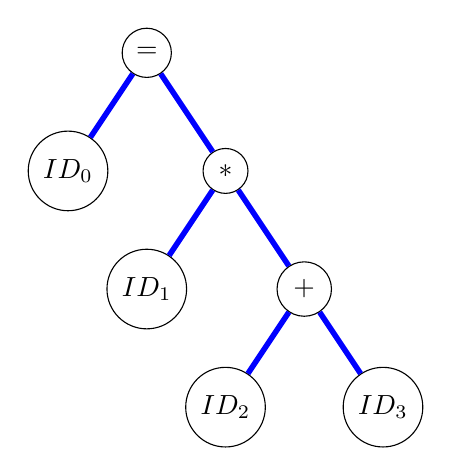
\begin{tikzpicture}
 	\node[draw,circle] (N0) at (1,4.5) {$=$};
 	\node[draw,circle] (N1) at (0,3) {$ID_0$};
 	\node[draw,circle] (N2) at (2,3) {$\ast$};
 	\node[draw,circle] (N3) at (1,1.5) {$ID_1$};
 	\node[draw,circle] (N4) at (3,1.5) {$+$};
 	\node[draw,circle] (N5) at (2,0) {$ID_2$};
 	\node[draw,circle] (N6) at (4,0) {$ID_3$};
 	\path[-,color=blue,line width=2pt] (N0) edge (N1)
 	     (N0) edge (N2)  (N2) edge (N3)
 	     (N2) edge (N4)  (N4) edge (N5)
 	     (N4) edge (N6);
 \end{tikzpicture}
} &\quad &
\scalebox{0.75}{
	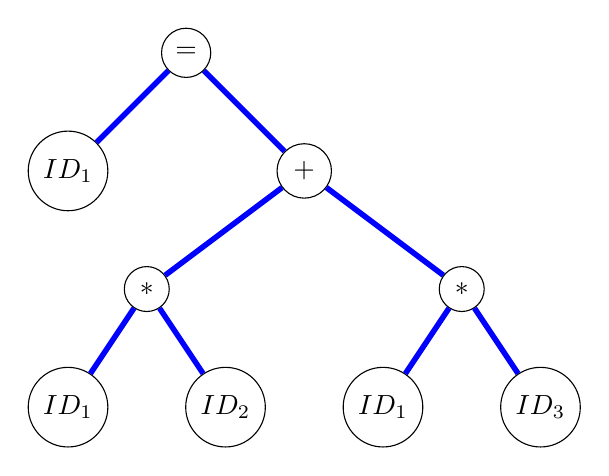
\begin{tikzpicture}
	\node[draw,circle] (N0) at (1.5,4.5) {$=$};
	\node[draw,circle] (N1) at (0,3) {$ID_1$};
	\node[draw,circle] (N2) at (3,3) {$+$};
	\node[draw,circle] (N3) at (1,1.5) {$\ast$};
	\node[draw,circle] (N4) at (5,1.5) {$\ast$};
	\node[draw,circle] (N5) at (0,0) {$ID_1$};
	\node[draw,circle] (N6) at (2,0) {$ID_2$};
	\node[draw,circle] (N7) at (4,0) {$ID_1$};
	\node[draw,circle] (N8) at (6,0) {$ID_3$};
	\path[-,color=blue,line width=2pt]
	     (N0) edge (N1)  (N0) edge (N2)
	     (N2) edge (N3)  (N2) edge (N4)
	     (N3) edge (N5)  (N3) edge (N6)
	     (N4) edge (N7)  (N4) edge (N8);
	\end{tikzpicture}

}
\end{tabular}
\end{frame}

\begin{frame}
 \frametitle{3番地コード}
 \[
 \begin{array}{lp{.5\textwidth}}
  C = A\theta B & $+$,$-$,$*$,$/$,$\mathsf{and}$,$\mathsf{or}$,$>$,$>=$,$=$,$!=$,$<=$,$<$\\[5pt]
  B = \theta A & $-$,$\mathsf{not}$\\[5pt]
  B = A\\[5pt]
  \multicolumn{2}{l}{\mbox{\greentext{Jump on condition}}}\\[5pt]
  \multicolumn{2}{l}{\mathtt{if}\ A\ \mathtt{goto}\ L}\\[5pt]
  \multicolumn{2}{l}{\mathtt{if}\ not A\ \mathtt{goto}\ L}\\[5pt]
  \multicolumn{2}{l}{\mbox{\greentext{Unconditional Jump}}}\\[5pt]
  \multicolumn{2}{l}{\mathtt{goto}\ L}
 \end{array}
 \]
\end{frame}

\begin{frame}
  \frametitle{抽象構文木からの３番地コード生成}
  \begin{tabularx}{\textwidth}{XX}
    \multicolumn{1}{m{.5\textwidth}}{
      \begin{tabularx}{.5\textwidth}{X}
  $ID_0=ID_1\ast(ID_2+ID_3)$\\[25pt]
  $\begin{array}{l}
    \uncover<2->{t_1=ID_0}\\
    \uncover<3->{t_3=ID_1}\\
    \uncover<4->{t_5=ID_2}\\
    \uncover<5->{t_6=ID_3}\\
    \uncover<6->{t_4=t_5+t_6}\\
    \uncover<7->{t_2=t_3\ast t_4}\\
    \uncover<8->{t_7=(t_1=t_6)}
  \end{array}$
\end{tabularx}
    }
&
\multicolumn{1}{m{.4\textwidth}}{
  \scalebox{0.75}{
    \begin{tikzpicture}
      \node[draw,circle,label={135:{$t_0$}}] (N0) at (1,4.5) {$=$};
      \node[draw,circle,label={135:{$t_1$}}] (N1) at (0,3) {$ID_0$};
      \node[draw,circle,label={45:{$t_2$}}] (N2) at (2,3) {$\ast$};
      \node[draw,circle,label={135:{$t_3$}}] (N3) at (1,1.5) {$ID_1$};
      \node[draw,circle,label={45:{$t_4$}}] (N4) at (3,1.5) {$+$};
      \node[draw,circle,label={135:{$t_5$}}] (N5) at (2,0) {$ID_2$};
      \node[draw,circle,label={45:{$t_6$}}] (N6) at (4,0) {$ID_3$};
      \path[-,color=blue,line width=2pt] (N0) edge (N1)
           (N0) edge (N2)  (N2) edge (N3)
           (N2) edge (N4)  (N4) edge (N5)
           (N4) edge (N6);

    \only<2->{\draw[->,color=red,line width=2pt] (0.8,4.5) -- (-0.2,3.2);}
    \only<3->{\draw[color=red,line width=2pt] (0.2,2.8) to[in=180] (1,4);
    \draw[color=red,line width=2pt] (1,4) to[out=0,in=90] (1.6,3);
    \draw[->,color=red,line width=2pt] (1.6,3) to [out=270,in=60] (1,1.7);
    }
    \only<4->{\draw[color=red,line width=2pt] (1.2,1.7) to [in=180] (2,2.5);
    \draw[color=red,line width=2pt](2,2.5) to [out=0,in=90] (2.6,1.5);
    \draw[->,color=red,line width=2pt](2.6,1.5) to [out=270,in=60] (2,0.2);}
    \only<5->{\draw[color=red,line width=2pt] (2.2,0.2) to [in=180] (3,1);
    \draw[->,color=red,line width=2pt] (3,1) to [out=0,in=120] (3.7,0.2);}
    \only<6->{\draw[->,color=red,line width=2pt] (4,0.3) -- (3.3,1.3);}
    \only<7->{\draw[->,color=red,line width=2pt] (3,1.8) -- (2.2,2.8);}
    \only<8->{\draw[->,color=red,line width=2pt] (2,3.2) -- (1.3,4.5);}
    \end{tikzpicture}
   }}
  \end{tabularx}
\begin{center}
  \only<1>{\greentext{抽象構文木に一時変数$t_i$を割り当てる}}
  \only<2>{\greentext{ポストオーダーでトレースし，$t_1=ID_0$を生成}}
  \only<3>{\greentext{ポストオーダーでトレースし，$t_3=ID_1$を生成}}
  \only<4>{\greentext{ポストオーダーでトレースし，$t_5=ID_2$を生成}}
  \only<5>{\greentext{ポストオーダーでトレースし，$t_6=ID_3$を生成}}
  \only<6>{\greentext{ポストオーダーでトレースし，$t_4=t_5 + t_6$を生成}}
  \only<7>{\greentext{ポストオーダーでトレースし，$t_2=t_3 \ast t_4$を生成}}
  \only<8>{\greentext{ポストオーダーでトレースし，$t_0=(t_1 = t_2)$を生成}}
\end{center}
\end{frame}

% \begin{frame}
%  \frametitle{スタックマシンによる3番地コード}
%  $C=A\theta B$\\
%  逆ポーランド記法:$\mbox{push A},\mbox{push B},\theta$\\
%  \quad スタックトップを$C$に格納
%  \[
%  \begin{array}{cccccc}
%   \begin{array}{|c|}
%    \ \\\hline
%    A \\\hline
%   \end{array} & \rightarrow &
%   \begin{array}{|c|}
%    \ \\\hline
%    B \\\hline
%    A \\\hline
%   \end{array} & \rightarrow &
%   \begin{array}{|c|}
%    \ \\\hline
%    C \\\hline
%   \end{array} & \\
%   \mbox{push A} & & \mbox{push B} & & \multicolumn{2}{l}{\mbox{pop};\mbox{pop};\theta;\mbox{push C}}
%  \end{array}
%  \]
 
%  \begin{trivlist}
%    \item 単純に実行可能で抽象構文木をポストオーダーでトラバースすることで中間コード生成が可能。
%    \item 最適化のコストが大きい
%    \item スタックマシンの考え方に基づいて中間コードを生成する
%    \item 演算対象となるメモリを抽象的に指定する（静的単一代入）
%  \end{trivlist}
% % \begin{center}
% %  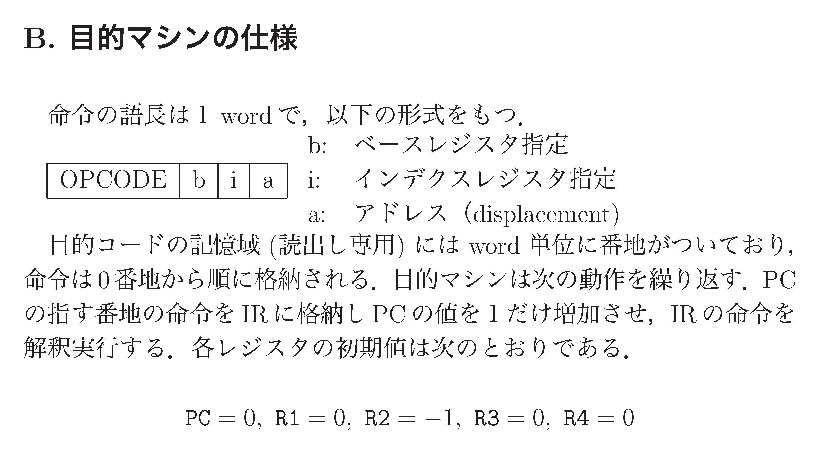
\includegraphics[scale=0.6]{inst00.eps}
% % \end{center}
% \end{frame}

\begin{frame}[fragile]
  \frametitle{手続き呼び出しの3番地コード}
  \begin{center}
  \begin{tabularx}{.9\textwidth}{XX}
    \multicolumn{1}{m{.4\textwidth}}{
      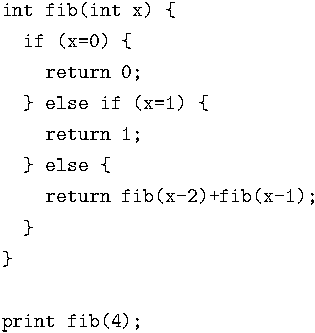
\includegraphics[scale=0.6]{fib_src-crop.pdf}
    }
    & 
    \multicolumn{1}{m{.4\textwidth}}{
      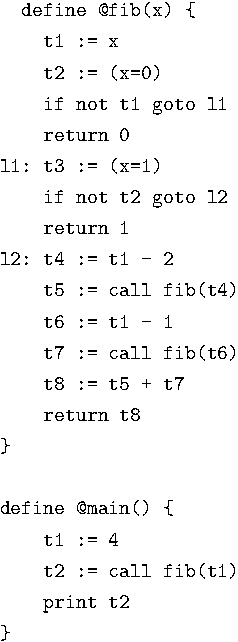
\includegraphics[height=0.75\textheight]{fib_3add-crop.pdf}
    }
  \end{tabularx}
\end{center}
{\small\color[rgb]{0,0.5,0}
{\begin{tabular}{l}定義：\verb|define @|関数名(仮引数リスト)\\
呼出：\verb|call @|関数名(実引数リスト)\end{tabular}}}
\end{frame}

% \begin{frame}[fragile]
% \frametitle{LLVM-IR}
% \begin{Verbatim}[fontsize=\scriptsize,label=HelloWorld.c,frame=single,numbers=left,numbersep=2pt]
% #include <stdio.h>
% int main() {
%   printf("HelloWorld\n");
%   return 0;
% }
% \end{Verbatim}

% \vspace*{5pt}

% \begin{Verbatim}[fontsize=\scriptsize,frame=single,showspaces=true]
% clang -emit-llvm -S -o HelloWorld.ll HelloWorld.c
% \end{Verbatim}

% \vspace*{5pt}

% \begin{Verbatim}[fontsize=\tiny,frame=single,label={\scriptsize HelloWorld.ll},numbers=left,numbersep=2pt]
% @.str = private unnamed_addr constant [13 x i8] c"Hello World\0A\00", align 1

% ; Function Attrs: noinline nounwind optnone ssp uwtable
% define i32 @main() #0 {
%   %1 = alloca i32, align 4
%   store i32 0, i32* %1, align 4
%   %2 = call i32 (i8*, ...) @printf(i8* getelementptr inbounds 
%                  ([13 x i8], [13 x i8]* @.str, i32 0, i32 0))
%   ret i32 0
% }

% declare i32 @printf(i8*, ...) #1
% \end{Verbatim}
% \end{frame}

%
%
%\begin{frame}
% \frametitle{演習コンパイラのコード}
% \only<1>{
% \begin{center}
%  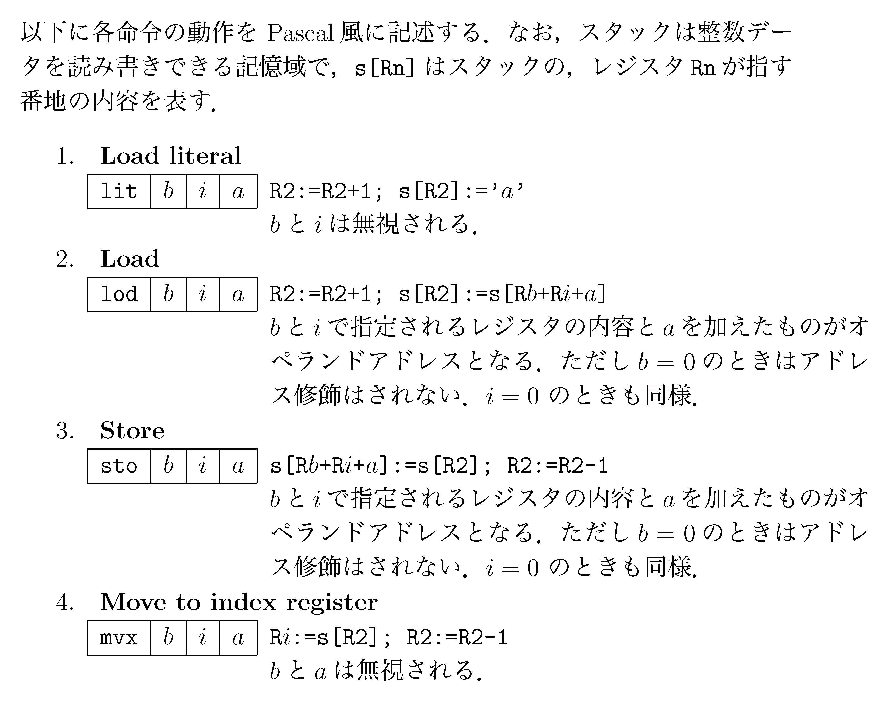
\includegraphics[scale=0.6]{inst01.eps}
% \end{center}
% }
% \only<2>{
% \begin{center}
%  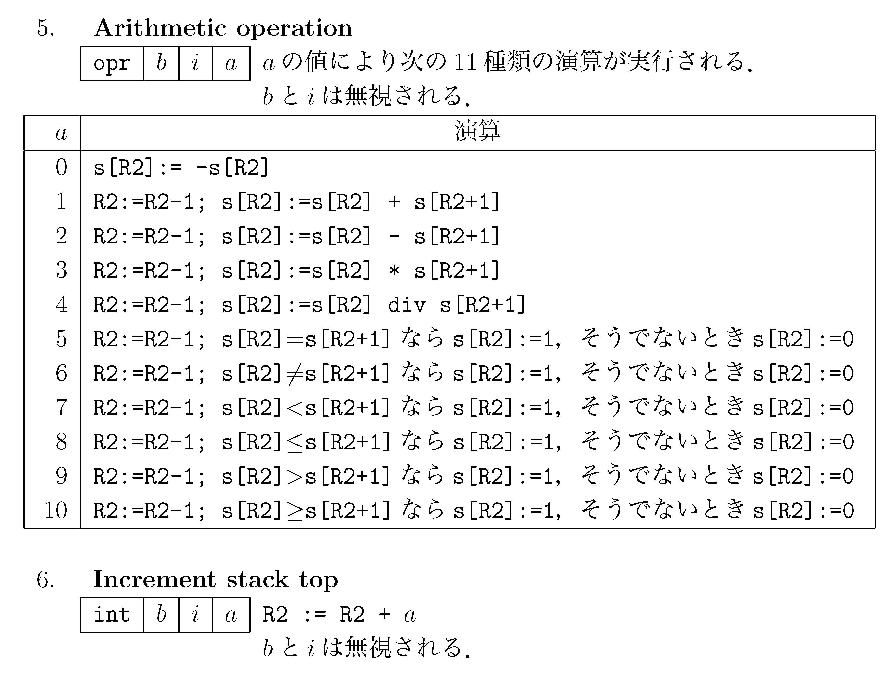
\includegraphics[scale=0.6]{inst02.eps}
% \end{center}
% }
% \only<3>{
% \begin{center}
%  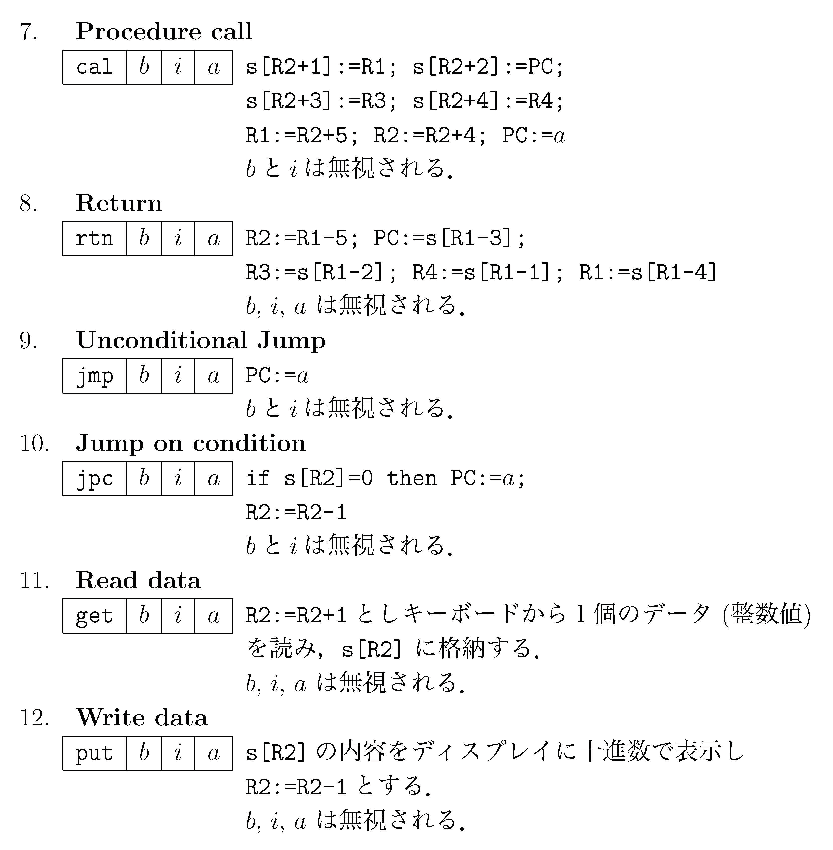
\includegraphics[scale=0.5]{inst03.eps}
% \end{center}
% }
%\end{frame}

% \begin{frame}
% \frametitle{LLVM-IRの命令\footnote{「きつねさんでもわかるLLVM」から引用}(メモリアクセス1)
% }
% {\scriptsize
% \begin{tabularx}{\textwidth}{|l|X|X|}\hline
% {\tt alloca} & 
%   result=alloca$\langle$type$\rangle$\newline
%     \quad [,$\langle$type$\rangle$ $\langle$NumElements$\rangle$]\newline
%     \quad [,align$\langle$alignment$\rangle$]
% & メモリ確保命令\newline type $\times$ NumElementsの領域を関数のスタックフレーム上に確保\\\hline
% {\tt load} & 
%   result=load [volatile]\newline
%   \quad $\langle$type$\rangle^\ast$ $\langle$pointer$\rangle$\newline
%   \quad [,align$\langle$alignment$\rangle$]\newline
%   \quad [,!nontemporal!$\langle$index$\rangle$]\newline
%   \quad [,!invariant.load !$\langle$index$\rangle$]\newline 
%   result=load atomic [volatile]\newline
%   \quad $\langle$type$\rangle^\ast$ $\langle$pointer$\rangle$\newline
%   \quad $\langle$singlethread$\rangle$ $\langle$ordering$\rangle$\newline
%   !index=! i32 1\newline
%   \quad align $\langle$alignment$\rangle$
% & ロード命令\newline
%     pointerが指すメモリアドレスから値を読み出す\newline
%     volatileが指定されている場合、最適化はload命令の実行順や実行数をほかのvolatileな命令に変更することができない\\\hline
% \end{tabularx}
% }
% \end{frame}

% \begin{frame}{LLVM-IRの命令(メモリアクセス2)}

% {\scriptsize 
% \begin{tabularx}{\textwidth}{|l|X|X|}\hline
% {\tt store} &
%   store [volatile]\newline
%   \quad $\langle$type$\rangle$ $\langle$value$\rangle$\newline
%   \quad $\langle$type$\rangle^\ast$ $\langle$pointer$\rangle$\newline
%   \quad [,align $\langle$alignment$\rangle$]\newline
%   \quad [,!nontemporal !$\langle$index$\rangle$]\newline
%   store atomic [volatile]\newline
%   \quad $\langle$type$\rangle$ $\langle$value$\rangle$\newline
%   \quad $\langle$type$\rangle^\ast$ $\langle$pointer$\rangle$\newline
%   \quad [singlethread] $\langle$ordering$\rangle$\newline
%   \quad align $\langle$alignment$\rangle$
%   & ストア命令\newline poinerが指すメモリアドレスに値を格納する\newline volatileが指定されている場合、最適化はstore命令の実行順や実行数をほかのvolatileな命令に変更することができない\\\hline
%   {\tt getelementptr} &
%   result = getelemntptr\newline
%   \quad $\langle$ptyple$\rangle^\ast$ $\langle$ptrval$\rangle$\newline
%   \quad \{, $\langle$type$\rangle$ $\langle$idx$\rangle$ \}$^\ast$\newline
%   result = getelementptr inbounds\newline
%   \quad $\langle$ptyple$\rangle^\ast$ $\langle$ptrval$\rangle$\newline
%   \quad \{, $\langle$type$\rangle$ $\langle$idx$\rangle$ \}$^\ast$\newline
%   result = getelementptr\newline
%   \quad $\langle$ptr vector$\rangle$,\newline
%   \quad $\langle$vector index type$\rangle$ $\langle$idex$\rangle$
%   &
%   要素アドレス取得命令\newline
%   合成型内の要素のアドレスを計算する\newline
%   prtvalが指す青dレスをベースとしてidxで指定したインデックスの要素アドレスを計算する\\\hline
% \end{tabularx}
% }
% \end{frame}

% \begin{frame}
% \frametitle{LLVM-IRの命令(演算命令)}
% {\scriptsize
% \begin{tabularx}{\textwidth}{|l|X|X|}\hline
% {\tt add} & {\tiny
% result = add $\langle$type$\rangle$ $\langle$op1$\rangle$ $\langle$op2$\rangle$	\newline
% result = add nuw $\langle$type$\rangle$ $\langle$op1$\rangle$ $\langle$op2$\rangle$	\newline
% result = add nsw $\langle$type$\rangle$ $\langle$op1$\rangle$ $\langle$op2$\rangle$	\newline
% result = add nuw nsw $\langle$type$\rangle$ $\langle$op1$\rangle$ $\langle$op2$\rangle$}
% &
% 加算命令\newline op1とop2を加算して結果を返す。op1, op2は整数か整数のベクタ。\newline
% nuw = No Unsigned Wrap, nsw = No Signed Wrap/ オーバーフローが発生したときに結果が未定義\\\hline
% \end{tabularx}
% }

% \vspace*{10pt}

% 同様な演算命令 fadd, sub, fsub, mul, fmul, udiv, sdiv, fdiv, urem,srem,frem(剰余)
% \end{frame}

% \begin{frame}
% \frametitle{LLVM-IRの命令(制御命令)}
% {\scriptsize
% \begin{tabularx}{\textwidth}{|l|X|X|}\hline
% {\tt ret} & 
% ret $\langle$type$\rangle$ $\langle$value$\rangle$\newline ret void
% &
% return 命令\newline
% 関数の呼び出し元へ制御を戻す\newline
% valueが指定されていればvalueを戻す
% \\\hline
% {\tt br} &
% br i1 $\langle$cond$\rangle$, label $\langle$iftrue$\rangle$, label $\langle$iffalse$\rangle$\newline
% br label $\langle$dest$\rangle$
% &
% 分岐命令\newline
% condのtrue/falseに応じて分岐先が変わる\newline
% condが指定されない場合はラベルdestに無条件分岐する\\\hline
% \end{tabularx}
% }

% \vspace*{10pt}

% {\scriptsize
% \begin{tabularx}{\textwidth}{|l|X|X|}\hline
% {\tt icmp} & 
% result=icmp $\langle$cond$\rangle$ $\langle$type$\rangle$ $\langle$op1$\rangle$ $\langle$op2$\rangle$
% &
% 比較命令\newline
% op1, op2をcondで指定した条件で比較し、真偽を返す。op1, op2は整数、ポインタか整数のベクトル\\\hline
% {\tt call} &
% result = [tail] call [cconv] [ret attrs] $\langle$type$\rangle$\newline
% \quad [$\langle$ fnty$\rangle^\ast$] $\langle$fnptrval$\rangle$\newline
% \quad ($\langle$function args$\rangle$)[fn attrs]
% &
% 関数呼び出し命令\newline
% 関数fnptrvalをfunction argsを引数として呼び出す。\\\hline
% \end{tabularx}
% }

% \end{frame}

% \begin{frame}
% \frametitle{LLVM-IRの命令(cond)}
% {\scriptsize
% \begin{tabularx}{\textwidth}{|l|X|}\hline
% {\tt eq} & 
% equal ２つの引数が同値の場合true, それ以外false\\\hline
% {\tt ne} & equalの否定\\\hline
% {\tt ugt} & ２つの引数をunsigned valueとして扱って第一引数が第二引数よりも大きい場合にtrue, それ以外false\\\hline
% {\tt uge} & ２つの引数をunsigned valueとして扱って第一引数が第二引数よりも大きいか同じ場合にtrue, それ以外false\\\hline
% {\tt ult} & ２つの引数をunsigned valueとして扱って第一引数が第二引数よりも小さい場合にtrue, それ以外false\\\hline
% {\tt ule} & ２つの引数をunsigned valueとして扱って第一引数が第二引数よりも小さいか同じ場合にtrue, それ以外false\\
% {\tt sgt} & ２つの引数をunsigned valueとして扱って第一引数が第二引数よりも大きい場合にtrue, それ以外false\\\hline
% {\tt sge} & ２つの引数をunsigned valueとして扱って第一引数が第二引数よりも大きいか同じ場合にtrue, それ以外false\\\hline
% {\tt slt} & ２つの引数をunsigned valueとして扱って第一引数が第二引数よりも小さい場合にtrue, それ以外false\\\hline
% {\tt sle} & ２つの引数をunsigned valueとして扱って第一引数が第二引数よりも小さいか同じ場合にtrue, それ以外false\\\hline
% \end{tabularx}
% }
% \end{frame}



% \begin{frame}[fragile]
%  \frametitle{例}
%  \begin{tabularx}{\textwidth}{XX}
%   \multicolumn{1}{m{.5\textwidth}}{
%     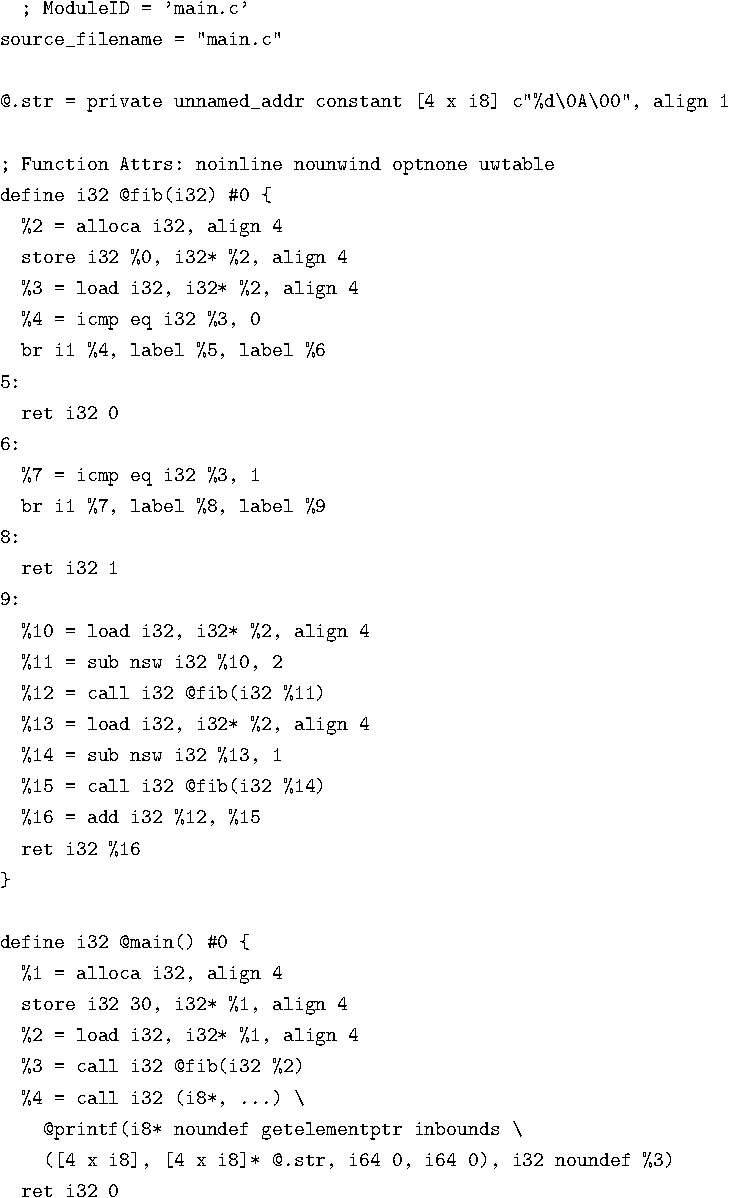
\includegraphics[scale=0.5]{fib_llvm-crop.pdf}
%   } & 
%   \multicolumn{1}{m{.5\textwidth}}{
%     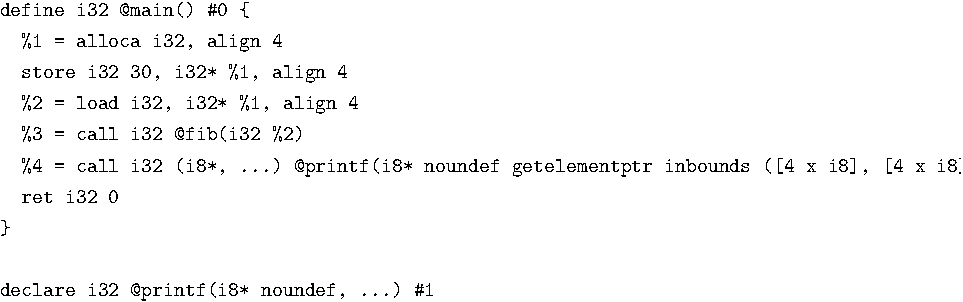
\includegraphics[scale=0.5]{fib_llvm2-crop.pdf}
%   }
% %  \begin{minipage}{.4\textwidth}
% % 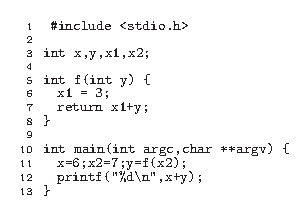
\includegraphics{Prog1_7_c.eps}
% % \vspace*{7cm}
% % \end{minipage}
% % &
% % 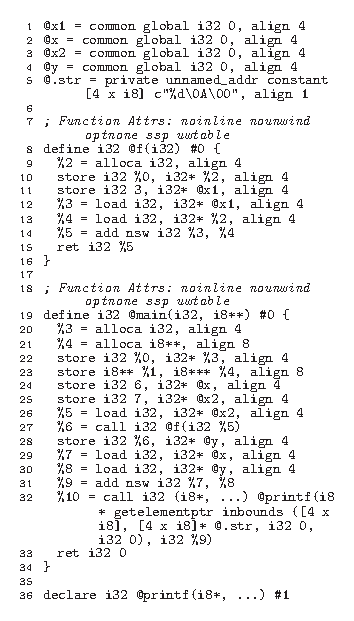
\includegraphics[height=.8\textheight]{Prog1_7_ll.eps}
% \end{tabularx}

% \end{frame}

\subsection{実行時環境}

\begin{frame} 
 \frametitle{実行時環境}
 \greentext{メモリ領域の割り当て方}

 \begin{tabular}{ccc}
 \begin{minipage}{.5\textwidth}
 \begin{list}{$\bullet$}{}
  \item 大域変数=ヒープ領域(\greentext{プロセス内のメモリ領域})にわりあ
	てる。\\
	{\tt malloc},{\tt free}\\
	演習のコンパイラでは、スタック領域の底にわりあてる(popしない)。
  \item 局所変数=スタックにわりあてる
  \item 関数・手続の引数のわりあて(特殊な局所変数)
 \end{list}
 \end{minipage} & \quad &
 \begin{minipage}{.5\textwidth}
 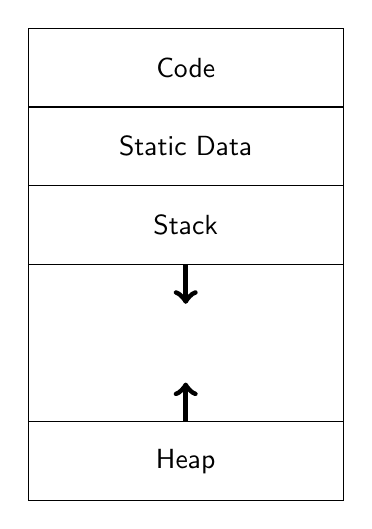
\begin{tikzpicture}
 	\draw (0,0) rectangle (4,6);
 	\node at (2,5.5) {Code};
 	\draw (0,5) -- (4,5);
 	\node at (2,4.5) {Static Data};
 	\draw (0,4) -- (4,4);
 	\node at (2,3.5) {Stack};
 	\draw (0,3) -- (4,3);
 	\draw (0,1) -- (4,1);
 	\node at (2,0.5) {Heap};
 	\draw [->,line width=2pt] (2,1) -- (2,1.5);
 	\draw [->,line width=2pt] (2,3) -- (2,2.5);
 \end{tikzpicture}
 \end{minipage}
 \end{tabular}
\end{frame}

\begin{frame}
 \frametitle{静的割当てと動的割当て}
 \begin{tabular}{cc}
  \begin{minipage}{.5\textwidth}
   \begin{list}{}{}
    \item 静的割当て:
	  \greentext{\small 実行の最初から最後までメモリ領域が変化しない}
    \item 動的割り当て：
	  \greentext{\small メモリ領域が実行時に決定}\\
	  \greentext{\small 実行終了時に領域が不要になる}
   \end{list}
  \end{minipage} 
 &
  \begin{minipage}{.5\textwidth}
   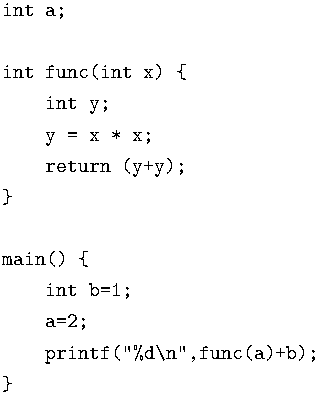
\includegraphics[scale=.75]{prog1.pdf}
  \end{minipage}
 \end{tabular}
 
 \begin{center}
 \begin{list}{}{}
  \item 静的割当て: {\tt a},{\tt func},{\tt main}
  \item 動的割当て: {\tt x},{\tt y},{\tt b}
 \end{list}
 \end{center}
\end{frame}

\subsection{駆動レコード}

\begin{frame}
 \frametitle{駆動レコード}
 手続き/関数の一回の実行に必要な局所情報\\
 \greentext{PC(Program Counter)、返り値、参照可能なシンボルの集合}

 \begin{center}
 \begin{tikzpicture}
    \draw[style=dotted] (3.5,2) -- (7.5,2);
    \draw[style=dotted] (3.5,1.5) -- (7.5,1.5);
 
 	\draw (0,0) rectangle (1.5,1.5);
 	\draw (0,0.5) -- (1.5,0.5);
 	\draw (0,1) -- (1.5,1);
 	\draw (1,1.5) -- (1,0);
 	\node at (0.75,-.3) {実行前};
 	\node at (0.5,0.25) {a};
 	\node at (0.5,0.75) {func};
 	\node at (0.5,1.25) {main};
 	
 	\draw (2,0) rectangle (3.5,2);
 	\draw (2,0.5) -- (3.5,0.5);
 	\draw (2,1) -- (3.5,1);
 	\draw (2,1.5) -- (3.5,1.5);
 	\draw (3,2) -- (3,0);
 	\node at (2.75,-.3) {main実行中};
 	
 	\node at (2.5,0.25) {a};
 	\node at (2.5,0.75) {func};
 	\node at (2.5,1.25) {main};
 	\node at (2.5,1.75) {b};
 	
 	\draw (4,0) rectangle (5.5,3);
 	\draw (4,0.5) -- (5.5,0.5);
 	\draw (4,1) -- (5.5,1);
 	\draw (4,1.5) -- (5.5,1.5);
 	\draw (4,2) -- (5.5,2);
 	\draw (4,2.5) -- (5.5,2.5);
 	\draw (5,0) -- (5,3);
 	\node at (4.75,-.3) {func実行中};

 	\node at (4.5,0.25) {a};
 	\node at (4.5,0.75) {func};
 	\node at (4.5,1.25) {main};
 	\node at (4.5,1.75) {b};
	\node at (4.5,2.25) {x};
	\node at (4.5,2.75) {y}; 	
 	
 	\node at (7,0.75) {大域変数};
 	\node at (7.5,1.75) {mainのレコード};
 	\node at (7.5,2.5) {funcのレコード};
\end{tikzpicture}
 \end{center}

% \begin{center}
%  \includegraphics{activationRec1.eps}
% \end{center}
\end{frame}

\begin{frame}
 \frametitle{駆動レコードの構成}
 
 \begin{tikzpicture}
 	\draw (0,0) rectangle (4,4.8);
 	\draw (0,0.6) -- (4,0.6);
 	\draw (0,1.2) -- (4,1.2);
 	\draw (0,1.8) -- (4,1.8);
 	\draw (0,2.4) -- (4,2.4);
 	\draw (0,3) -- (4,3);
 	\draw (0,3.6) -- (4,3.6);
 	\draw (0,4.2) -- (4,4.2);
 	\node at (2,4.5) {一時変数領域};
 	\node at (2,3.9) {局所データ領域};
 	\node at (2,3.3) {静的リンク};
 	\node at (2,2.7) {動的リンク};
 	\node at (2,2.1) {戻り番地};
 	\node at (2,1.5) {実引数計算領域};
 	\node at (2,0.9) {戻り値};
 	\node at (2,0.3) {退避領域};
 	\draw[->] (4.5,2.7) -- (4,2.7);
 	\node at (5,2.7) {FP};
 	
 	\node[anchor=west] at (5.5,4.5) {\greentext{関数内での計算の一時領域}};
    \node[anchor=west] at (5.5,3.9) {\greentext{局所宣言された変数の領域}};
    \node[anchor=west] at (5.5,3.3) {\greentext{次に外へ参照すべきレコード}};
    \node[anchor=west] at (5.5,2.7) {\greentext{Return後に復元すべきレコード}};
    \node[anchor=west] at (5.5,2.1) {\greentext{Return後に再開するPC}};
    \node[anchor=west] at (5.5,1.5) {\greentext{呼出の際に引数受け渡しに使う}};
    \node[anchor=west] at (5.5,0.9) {\greentext{関数の計算結果を格納}};
    \node[anchor=west] at (5.5,0.3) {\greentext{呼出の際の一時領域}};
 \end{tikzpicture}
 
% \begin{pspicture}(0,0)(3,5)
%  \psframe(0,0)(3,4)
%  \rput(1.5,3.75){一時変数領域}
%  \psline(0,3.5)(3,3.5)
%  \rput(1.5,3.25){局所データ領域}
%  \psline(0,3)(3,3)
%  \rput(1.5,2.75){静的リンク}
%  \psline(0,2.5)(3,2.5)
%  \rput(1.5,2.25){動的リンク}
%  \psline(0,2)(3,2)
%  \rput(1.5,1.75){戻り番地}
%  \psline(0,1.5)(3,1.5)
%  \rput(1.5,1.25){実引数計算領域}
%  \psline(0,1)(3,1)
%  \rput(1.5,0.75){戻り値}
%  \psline(0,0.5)(3,0.5)
%  \rput(1.5,0.25){退避領域}
%  \pnode(3,2.25){P1}
%  \pnode(3.5,2.25){P2}
%  \ncline{<-}{P1}{P2}
%  \rput(4,2.25){FP}
% \end{pspicture}
% \begin{pspicture}(0,0)(4,5)
%  \rput[l](1.25,3.75){\greentext{関数内での計算の一時領域(×)}}
%  \rput[l](1.25,3.25){\greentext{局所宣言された変数の領域}}
%  \rput[l](1.25,2.75){\greentext{\small スコープルールで次に外へ参照すべきレコード}}
%  \rput[l](1.25,2.25){\greentext{Return後に復元すべきレコード}}
%  \rput[l](1.25,1.75){\greentext{Return後に再開するPC}}
%  \rput[l](1.25,1.25){\greentext{呼出の際に引数受け渡しに使う(×)}}
%  \rput[l](1.25,0.75){\greentext{関数の計算結果を格納}}
%  \rput[l](1.25,0.25){\greentext{呼出の際の一時領域(×)}}
% \end{pspicture}
 
% \vspace*{2em}
%
% (×)のところは演習では利用しない.
% 動的リンクも不要
\end{frame}

% Insert demo

\newcommand{\commandPointer}[1]{\node[anchor=west,red] at ($#1*(0,0.5)+(-.45,0)$)  {$\rightarrow$};}

\begin{frame}[fragile]
 \frametitle{変数の参照}
 
 \begin{tikzpicture}
 	\node[anchor=west] at (0,6.5) 
 	  {\verb|int a;|};
 	\node[anchor=west] at (0,6.0) 
 	  {\verb|int func(int x) {|};
 	\node[anchor=west] at (0,5.5) 
 	  {\verb|  int y;|};
 	\node[anchor=west] at (0,5.0) 
 	  {\verb|  if(x==1) {return(a);}|};
 	\node[anchor=west] at (0,4.5)
 	  {\verb|  else {|};
 	\node[anchor=west] at (0,4.0)
 	  {\verb|    y=func(x-1)*2;|};
 	\node[anchor=west] at (0,3.5)
 	  {\verb|    return(a+y);|};
 	\node[anchor=west] at (0,3.0)
 	  {\verb|  }|};
 	\node[anchor=west] at (0,2.5)
 	  {\verb|}|};
 	\node[anchor=west] at (0,2.0)
 	  {\verb|void main() {|};
 	\node[anchor=west] at (0,1.5)
 	  {\verb|  a=2;|};
    \node[anchor=west] at (0,1.0)
      {\verb|  printf("func(3)=%d",|};
    \node[anchor=west] at (0,0.5)
      {\verb|    func(3));|};
    \node[anchor=west] at (0,0)
      {\verb|}|};
    \draw (-0.5,-0.5) rectangle +(6.5,7.5);
    
%    \only<2>{\node[anchor=west,red] at (-.45,1.5) {$\rightarrow$};}
%    \only<3>{\node[anchor=west,red] at (-.45,1.0) {$\rightarrow$};}
    \only<2>{\commandPointer{3}}
    \only<3>{\commandPointer{2}}
    \only<4>{\commandPointer{10}}
    \only<5>{\commandPointer{8}}
    \only<6>{\commandPointer{10}}
    \only<7>{\commandPointer{8}}
    \only<8,9>{\commandPointer{10}}
    \only<10,11,12>{\commandPointer{8}} 
    \only<13>{\commandPointer{7}}
    \only<14,15,16>{\commandPointer{8}}
    \only<17>{\commandPointer{7}}
    \only<18>{\commandPointer{3}}  

    \only<1-16>{\node at (9,1.5) {\tt ?};}    
    \only<1>{\node at (9,1) {\tt a=?};}
    \only<2->{\node at (9,1) {\tt a=2};}
    \only<4-17>{\node at (9,2) {\tt x=3};}
    \only<4-15>{\node at (9,2.5) {\tt y=?};}
    \only<4-17>{\draw (8,1.25) rectangle +(2,1.5);}
    \only<6-12>{\node at (9,3) {\tt ?};}
    \only<6-13>{\node at (9,3.5) {\tt x=2};}
    \only<6-11>{\node at (9,4) {\tt y=?};}
    \only<6-13>{\draw (8,2.75) rectangle +(2,1.5);}
    \only<8>{\node at (9,4.5) {\tt ?};}
    \only<8,9>{\node at (9,5) {\tt x=1};}
    \only<8,9>{\node at (9,5.5) {\tt y=?};}
    \only<8,9>{\draw (8,4.25) rectangle +(2,1.5);}
    \only<9,10>{\node at (9,4.5) {\tt 2};}
    \only<11>{\node at (9,4.5) {\tt 2*2};}
    \only<12,13>{\node at (9,4) {\tt y=4};}
    \only<13,14>{\node at (9,3) {\tt 6};}
    \only<15>{\node at (9,3) {\tt 6*2};}
    \only<16,17>{\node at (9,2.5) {\tt y=12};}
    \only<17,18>{\node at (9,1.5) {\tt 14};}
    
    \only<4-17>{\path[->,blue,line width=1.5pt] (8,2) edge [out=180,in=180] (8,1);}
    \only<6-13>{\path[->,blue,line width=1.5pt] (8,3.5) edge [out=180,in=180] (8,1);}
    \only<8,9>{\path[->,blue,line width=1.5pt] (8,5) edge [out=180,in=180] (8,1);}
    \only<4-17>{\node at (9,0) {\color{blue}静的リンク};}
 \end{tikzpicture}
\end{frame}

\begin{frame}
 \frametitle{変数の参照/記憶位置の決定}

 \begin{list}{}{}
  \item 局所変数: フレームポインタからの相対位置
  \item 大域変数: ヒープ内のアドレス\\
%	(実習)：スタックボトムからの相対位置
 \end{list}

% (実習)動的変数の位置：何番目に宣言されているか\\
 
 記号表にはスタックレームレジスタからの相対番地=何番目に宣言でどういった
 型をもつか。

 型情報=確保する領域量(実習の場は整数のみ)

 関数の引数うけわたしは局所変数の宣言+代入
	
\end{frame}

\section{構文主導型変換}

\subsection{意味解析}

\begin{frame}{動作意味}
\[\langle\{S,E,T,F\},\{+,\ast,(,),n\},P,S
  \rangle\]
  \[\left\{\begin{array}{ll}
    S\rightarrow E\#, & T\rightarrow F,\\
    E\rightarrow E+T, & F\rightarrow (\ E\ ),\\
    E\rightarrow T, & F\rightarrow n,\\
    T\rightarrow T\ast F & \\
  \end{array}\right\}\]

  \vspace*{3mm}

  \greentext{各生成規則は値を計算する意味を持つ．}

  \vspace*{3mm}

  $E\rightarrow E+T$: 右辺の$E$の値と$T$の値を加算した値を左辺の$E$の値とする．\\[3mm]
  $\Rightarrow$ \redtext{'+'に加算の意味を与える．}

\end{frame}

\begin{frame}{構文に従った動作意味}

  \[
    \begin{array}{ll}
      S\rightarrow E\# & var(S)= var(E)\\
      E\rightarrow E_1+T & var(E)= var(E_1)+var(T)\\
      E\rightarrow T & var(E)=var(T)\\
      T\rightarrow T_1\ast F & var(T)=var(T_1)\times var(F)\\
      T\rightarrow F & var(T)=var(T)\\
      F\rightarrow (\ E\ ) & var(F)=var(E)\\
      F\rightarrow i & temp=val(i);var(F)=temp
    \end{array}
  \]

  \vspace*{3mm}

  \greentext{構文主導型変換}

  \begin{description}
  \item [インタープリタ：] 生成規則に対応する動作をする．
  \item [コンパイラ：] 生成規則に対応した目的コード（中間コード）を生成する．
  \end{description}
\end{frame}

\subsection{中間コード生成ルーチン}


\begin{frame}
 \frametitle{構文主導型変換}
 CF文法の各生成規則に対してコード生成ルーチンをわりあてる。\\
 \begin{itemize}
  \item $\mathsf{newTemp}()$\\
	変数$T$の領域を確保して、記号番地または一時変数へのポインタを返す。
  \item $\mathsf{newLabel}()$\\
	新たなラベル名を返す。
  \item $\mathsf{generate}(\mbox{中間コード})$\\
	中間コードを出力ファイルに出力する。
 \end{itemize}

\greentext{
$n$回目に$\mathsf{newTemp}()$を呼びだしたとき、生成される
 変数$\texttt{t}n$}

\greentext{
$m$回目に$\mathsf{newLabel}()$を呼びだしたとき、生成されるラ
 ベル$\texttt{L}m$}

\end{frame}

\begin{frame}
 \frametitle{構文主導型変換の基礎}
 \begin{eqnarray*}
  S & \rightarrow & \mathsf{ID}\texttt{=}\ E\ \texttt{;}\\
  E & \rightarrow & E^{(1)}\ \texttt{+}\ \mathtt{NUM}\\
  E & \rightarrow & \mathtt{NUM}
 \end{eqnarray*}
 \begin{center}
 $\mathsf{ID}$\ $\texttt{=}$\ $\mathsf{NUM}_0$\ $\texttt{+}$\ $\mathsf{NUM}_1$
 \ $\texttt{+}$\ $\mathsf{NUM}_2$\ $\texttt{;}$
  \end{center}
\begin{center}
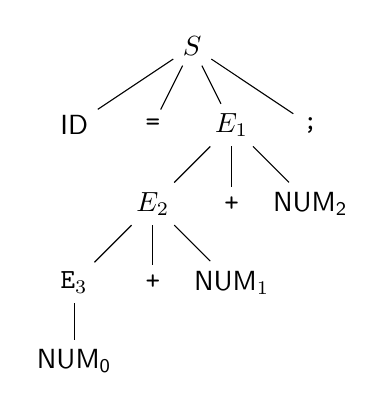
\begin{tikzpicture}
 \node (N0) at (0,0) {$\mathsf{NUM_0}$};
 \node (N1) at (0,1) {$\texttt{E}_3$};
 \node (N2) at (1,1) {$\texttt{+}$};
 \node (N3) at (2,1) {$\mathsf{NUM}_1$};
 \node (N4) at (1,2) {$E_2$};
 \node (N5) at (2,2) {$\texttt{+}$};
 \node (N6) at (3,2) {$\mathsf{NUM_2}$};
 \node (N7) at (0,3) {$\mathsf{ID}$};
 \node (N8) at (1,3) {$\texttt{=}$};
 \node (N9) at (2,3) {$E_1$};
 \node (N10) at (3,3) {$\texttt{;}$};
 \node (N11) at (1.5,4) {$S$};

 \path[-] (N0) edge (N1);
 \path[-] (N4) edge (N1) (N4) edge (N2) (N4) edge (N3);
 \path[-] (N9) edge (N4) (N9) edge (N5) (N9) edge (N6);
 \path[-] (N11) edge (N7) (N11) edge (N8) (N11) edge (N9) (N11) edge (N10);
\end{tikzpicture}
% \begin{pspicture}(0,0)(3,4)
%  \rput(1.5,4){\rnode{P0}{$S$}}
%  \rput(0,3){\rnode{P1}{$\mathsf{ID}$}}
%  \rput(1,3){\rnode{P2}{$\mathtt{'='}$}}
%  \rput(2,3){\rnode{P3}{$E_1$}}
%  \rput(3,3){\rnode{P4}{$\mathtt{';'}$}}
%  \rput(1,2){\rnode{P31}{$E_2$}}
%  \rput(2,2){\rnode{P32}{$\mathtt{'+'}$}}
%  \rput(3,2){\rnode{P33}{$\mathsf{NUM}_2$}}
%  \rput(0,1){\rnode{P311}{$E_3$}}
%  \rput(1,1){\rnode{P312}{$\mathtt{'+'}$}}
%  \rput(2,1){\rnode{P313}{$\mathsf{NUM}_1$}}
%  \rput(0,0){\rnode{P3111}{$\mathsf{NUM}_0$}}
%  \ncline{-}{P0}{P1}
%  \ncline{-}{P0}{P2}
%  \ncline{-}{P0}{P3}
%  \ncline{-}{P0}{P4}
%  \ncline{-}{P3}{P31}
%  \ncline{-}{P3}{P32}
%  \ncline{-}{P3}{P33}
%  \ncline{-}{P31}{P311}
%  \ncline{-}{P31}{P312}
%  \ncline{-}{P31}{P313}
%  \ncline{-}{P311}{P3111}
% \end{pspicture}

 \end{center}
\end{frame}

\begin{frame}
 \frametitle{中間コード(3番地コード)生成}
\begin{center}
  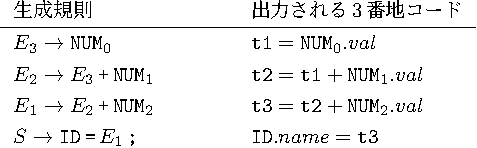
\includegraphics[scale=.8]{prodcode1-crop.pdf}
 \end{center} 
 \begin{center}
  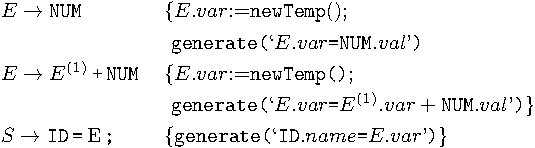
\includegraphics[scale=.8]{code-prog-r1-crop.pdf}
 \end{center} 
\end{frame}
\begin{frame}
 \frametitle{IF文の中間コード生成}
 \only<1>{
 \[
  \mbox{文}\ \rightarrow\ \mathsf{if}\ \mathtt{'('}\ \mbox{式}\
 \mathtt{')'}\ \mbox{文}^{(1)}
 \]
 \begin{enumerate}
  \item '式'のコードを生成 {\sf t1}に結果収納
  \item {\sf if not t1 goto l1}
  \item '文'$^{(1)}$のコードを生成
  \item {\sf l1:}
 \end{enumerate}
 }
 \only<2>{
 \[
  \mbox{文}\ \rightarrow\ \mathsf{if}\ \mathtt{'('}\ \mbox{式}\
 \mathtt{')'}\ \mbox{文}^{(1)}\ \mathsf{else}\ \mbox{文}^{(2)}
 \]
 \begin{enumerate}
  \item '式'のコードを生成 {\sf t1}に結果収納
  \item {\sf if not t1 goto l1}
  \item '文'$^{(1)}$のコードを生成
  \item {\sf goto l2}
  \item {\sf l1:}
  \item '文'$^{(2)}$のコードを生成
  \item {\sf l2:}
 \end{enumerate}
 }
\end{frame}
\begin{frame}
 \frametitle{while文の中間コード生成}
 \[
  \mbox{文}\ \rightarrow\ \mathsf{while}\ \mathtt{'('}\ \mbox{式}\
 \mathtt{')'}\ \mbox{文}^{(1)}
 \]
 \begin{enumerate}
  \item {\sf l1:}
  \item '式'のコードを生成 {\sf t1}に結果収納
  \item {\sf if not t1 goto l2}
  \item '文'$^{(1)}$のコードを生成
  \item {\sf goto l1}
  \item {\sf l2:}
 \end{enumerate}
\end{frame}


\begin{frame}
 \frametitle{構文主導型変換によるコード生成}
 {\small
 \begin{tabular}{lll}
  文$\rightarrow$ & {\tt if} ( & \{文.label:=\makenewlabel;\}\\
  & 式 & (式のコード)\\
  & )  & \{\genifnot{式.var}{文.label}\}\\
  & 文$^{(1)}$ & (文$^{(1)}$のコード)\{\genlabel{文.label};\\
  & & 文$^{(1)}$.label:=\makenewlabel;\gengoto{文$^{(1)}$.label}\}\\
  & {\tt else} & \{\genlabel{文.label}\}\\  
  & 文{$^{(2)}$} & \{\genlabel{文$^{(1)}$.label}\}
 \end{tabular}

\vspace*{1zw}

 \begin{tabular}{lll}
  文$\rightarrow$ & {\tt while} ( & \{文.label1:=\makenewlabel;\\
  & & \genlabel{文.label1}\} \\
  & 式 & (式のコード)\\
  & )  & \{文.label2:=\makenewlabel;\\
  &    & \genifnot{式.var}{文.label2}\}\\
  & 文$^{(1)}$ & (文のコード)\\
  &    & \{\gengoto{文.label1};\\
  &    & \genlabel{文.label2}\}\\
 \end{tabular}
 }
\end{frame}

% \section{記号表}

% \subsection{記号表}

% \begin{frame}
%  \frametitle{記号表}
% \begin{itemize}
%  \item 変数宣言：\greentext{記号定義}
%  \item 参照：\greentext{記号参照}
% \end{itemize}
%  定義によって得られる情報を記憶しておいて参照の際に利用する

%  \greentext{中間コードで変数になっていた部分に数値をわりあてる}

% \vspace*{10pt}

% \begin{tikzpicture}
%  \node (X0) at (0,0) {$x$};
%  \node (T0) at (0.5,0) {$:=$};
%  \node (X1) at (1,0) {$x$};
%  \node (T1) at (1.5,0) {$+$};
%  \node (X2) at (2,0) {$a$};
%  \node (I1) at (2.5,0) {$[$};
%  \node (X3) at (3,0) {$x$};
%  \node (I2) at (3.5,0) {$]$};
%  \node (E0) at (1,1) {$E$};
%  \node (E1) at (2.5,1) {$E$};
%  \node (E2) at (2,2) {$E$};
%  \node (S0) at (1,3) {$S$};

%  \path[-] (X0) edge (S0) (T0) edge (S0) (E2) edge (S0)
%           (E0) edge (E2) (T1) edge (E2) (E1) edge (E2)
%           (X1) edge (E0) 
%           (X2) edge (E1) (I1) edge (E1) (X3) edge (E1) (I2) edge (E1);

%  \draw[red] (0,0) circle (0.2);
%  \draw[red] (1,0) circle (0.2);
%  \draw[red] (3,0) circle (0.2);

%  \node[anchor=west] at (5,2.5) {\greentext{$x$は構文木上では無関係}};
%  \only<2>{\node[anchor=west] at (5,1) {\parbox{10zw}{\redtext{構文木上の要素の関連付けて同じアドレスを使ったコードを生成\newline $\Rightarrow$ 表に記録}}};}
% \end{tikzpicture}

% \end{frame}

% \begin{frame}
%  \frametitle{登録情報}
%  \begin{itemize}
%   \item 名前：\greentext{識別子}
%   \item 種類：\greentext{属性、関数名、変数名など}
%   \item 型：\greentext{記憶領域、引数の数、型}
%   \item 記憶位置：\greentext{スタック内での相対位置}
%  \end{itemize}
% \end{frame}

% \begin{frame}
%  \frametitle{データ構造}
%  \begin{itemize}
%   \item 線形リスト \greentext{配列：$O(n)$でアクセス}
%   \item ハッシュ表 教科書 5.2.2\\
% 	内部ハッシュ、外部ハッシュ
%   \item 二分木 \greentext{$O(\log_2(n))$でアクセス}
% 	データ+左ポインタ(自分より小さいエントリ)+右ポインタ(自分より大
% 	きいエントリ)
%  \end{itemize}
% \end{frame}

% \subsection{スコープルール}

% \begin{frame}
%  \frametitle{スコープルール}
%  スコープルール=識別子の有効範囲\\
%  \begin{trivlist}
%   \item C言語の場合：大域変数、ファイル内大域、関数内局所変数、プロック
% 	内局所変数
%   \item Java言語の場合：{\tt public}、{\tt protected}、{\tt private}、ブロック内局所
%  \end{trivlist}
% \end{frame}

% \begin{frame}
%  \frametitle{スコープルールの実現}
%  \greentext{演習のコンパイラ：厳密に1パス}
%  \begin{itemize}
%   \item 局所環境廃棄/復活の方法
%   \item 上書きのメカニズム
%  \end{itemize}
%  \greentext{局所変数を完全に上書きしてしまうと復活できなくなる}
 
%  解決法:
%  \begin{list}{}{}
%   \item 2以上同じ識別子のエントリを許して参照する順序を決める
%   \item 局所変数のラベルをつけて局所環境から出たら破棄\\
% 	(局所関数のレベルが1段階なので非常に単純)\\
% 	$\Rightarrow$教科書の場合はレベルを記号表に含めている。
%  \end{list}
% \end{frame}

%\begin{frame}
% \frametitle{VMの振舞い}
% \begin{center}
%   \begin{tabular}{p{.55\textwidth}p{.45\textwidth}}
%   \begin{minipage}{0.55\textwidth}
%   \only<1-2>{
%    \begin{pspicture}(0,0)(5,7)
%     \psframe(-0.5,0)(5,7)
%     \normalgap=0.375pt
%     \widegap=1.0pt
%     \indentval=0.4pt
%     \colpos=0.5pt
%     \rowheight=6.5pt
%     \fncstatline{program Example;}
%     \nnextline
%     \fncstatline{var a;}
%     \nnextline
%     \fncstatline{function func(x);}
%     \nnextline
%     \fncstatline{begin}
%     \nnextline\rindent
%     \fncstatline{var y;}
%     \nnextline
%     \fncstatline{if x=1 then}
%     \nnextline
%     \fncstatline{func:=a;}
%     \nnextline
%     \fncstatline{else begin}
%     \nnextline\rindent
%     \fncstatline{y:=func(x-1)*2;}
%     \nnextline
%     \fncstatline{func:=a+y;}
%     \nnextline\lindent
%     \fncstatline{end}
%     \nnextline\lindent
%     \fncstatline{end;}
%     \nnextline
%     \fncstatline{begin}
%     \nnextline\rindent
%     \fncstatline{a=2;}
%     \nnextline
%     \fncstatline{write(func(3));}
%     \nnextline\lindent
%     \fncstatline{end}
%    \end{pspicture}
%    }
%    \stackgap=0.32pt
%    \stackrowheight=0.5\stackgap
%    \framerowheight=1.5\stackgap
%    \gvarrowheight=1.5\stackgap
%    \newcount\stackheight\stackheight=25
%    \newcount\stacklinecnt
%    \newdimen\stackframerow
%    \newcommand{\stackframev}{\expandafter\Rval\the\stackframerow}
%    \only<3->{
%    \begin{pspicture}(0,0)(5,7)
%     \psline(1.5,0.32)(1.5,8.2)
%     \psline(3.5,0.32)(3.5,8.2)
%     {\stacklinecnt=0\relax\stackframerow=0pt
%     \loop
%     \advance\stacklinecnt1
%     \advance\stackframerow by \stackgap
%     \psline(1.5,\stackframev)(3.5,\stackframev)
%     \ifnum\stacklinecnt<\stackheight\repeat
%     }
%%%     \psline(1.5,0.4)(3.5,0.4)
%%     \psline(1.5,0.8)(3.5,0.8)\psline(1.5,1.2)(3.5,1.2)
%%     \psline(1.5,1.6)(3.5,1.6)\psline(1.5,2)(3.5,2)
%%     \psline(1.5,2.4)(3.5,2.4)\psline(1.5,2.8)(3.5,2.8)
%%     \psline(1.5,3.2)(3.5,3.2)\psline(1.5,3.6)(3.5,3.6)
%%     \psline(1.5,4)(3.5,4)\psline(1.5,4.4)(3.5,4.4)
%%     \psline(1.5,4.8)(3.5,4.8)\psline(1.5,5.2)(3.5,5.2)
%%     \psline(1.5,5.6)(3.5,5.6)\psline(1.5,6)(3.5,6)
%%     \psline(1.5,6.4)(3.5,6.4)
%%     \psline(1.5,6.8)(3.5,6.8)\psline(1.5,7.2)(3.5,7.2)
%%     \psline(1.5,7.6)(3.5,7.6)\psline(1.5,8)(3.5,8)
%     }
%     \only<3->{\intstackp{1}}\only<3>{\rarrows}
%     \only<4>{\rarrows}
%     \only<5->{\cpush}\only<5>{\showstacktop{2}}\only<5>{\rarrows}
%     \only<6->{\cpop}\only<6->{\ggstore{2}{0}}\only<6>{\rarrows}
%     \only<7->{\cpush}\only<7>{\showstacktop{3}}\only<7>{\rarrows}
%     \only<8-56>{\gstore{3}{5}}\only<8->{\cpop}\only<8>{\rarrows}
%     \only<9->{\cpush}\only<9>{\rarrows}
%     \only<10->{\callproc{1}}\only<10-56>{\callprocstack}\only<10>{\rarrows}
%     \only<11->{\intstackp{2}}\only<11>{\rarrows}
%     \only<12->{\cpush}\only<12-13>{\showstacktop{3}}\only<12>{\rarrows}
%     \only<13->{\cpush}\only<13>{\showstacktop{1}}\only<13>{\rarrows}
%     \only<14->{\cpop}\only<14>{\showstacktop{0}}\only<14>{\rarrows}
%     \only<15->{\cpop}\only<15>{\rarrows}
%     \only<16->{\cpush}\only<16-17>{\showstacktop{3}}\only<16>{\rarrows}
%     \only<17->{\cpush}\only<17>{\showstacktop{1}}\only<17>{\rarrows}
%     \only<18->{\cpop}\only<18>{\showstacktop{2}}\only<18>{\rarrows}
%     \only<19-48>{\gstore{2}{5}}\only<19->{\cpop}\only<19>{\rarrows}
%     \only<20->{\intstackp{1}}\only<20>{\rarrows}
%     \only<21->{\callproc{2}}\only<21-48>{\callprocstack}\only<21>{\rarrows}
%     \only<22->{\intstackp{2}}\only<22>{\rarrows}
%     \only<23->{\cpush}\only<23-24>{\showstacktop{2}}\only<23>{\rarrows}
%     \only<24->{\cpush}\only<24>{\showstacktop{1}}\only<24>{\rarrows}
%     \only<25->{\cpop}\only<25>{\showstacktop{0}}\only<25>{\rarrows}
%     \only<26->{\cpop}\only<26>{\rarrows}\only<26>{\rarrows}
%     \only<27->{\cpush}\only<27-28>{\showstacktop{2}}\only<27>{\rarrows}
%     \only<28->{\cpush}\only<28>{\showstacktop{1}}\only<28>{\rarrows}
%     \only<29->{\cpop}\only<29>{\showstacktop{1}}\only<29>{\rarrows}
%     \only<30-40>{\gstore{1}{5}}\only<30->{\cpop}\only<30>{\rarrows}
%     \only<31->{\intstackp{1}}\only<31>{\rarrows}
%     \only<32->{\callproc{2}}\only<32-40>{\callprocstack}\only<32>{\rarrows}
%     \only<33->{\intstackp{2}}\only<33>{\rarrows}
%     \only<34->{\cpush}\only<34-35>{\showstacktop{1}}\only<34>{\rarrows}
%     \only<35->{\cpush}\only<35>{\showstacktop{1}}\only<35>{\rarrows}
%     \only<36->{\cpop}\only<36>{\showstacktop{1}}\only<36>{\rarrows}
%     \only<37->{\cpop}\only<37>{\rarrows}
%     \only<38->{\cpush}\only<38>{\showstacktop{2}}\only<38>{\rarrows}
%     \only<39->{\cpop}\only<39-42>{\gstore{2}{-6}}\only<39>{\rarrows}
%     \only<40>{\rarrows}
%     \only<41->{\creturn{6}{7}}\only<41>{\rarrows}
%     \only<42->{\cpush}\only<42>{\showstacktop{2}}\only<42>{\rarrows}
%     \only<43->{\cpop}\only<43>{\showstacktop{4}}\only<43>{\rarrows}
%     \only<44->{\cpop}\only<44-48>{\showstacktop{4}}\only<44>{\rarrows}
%     \only<45->{\cpush}\only<45-46>{\showstacktop{2}}\only<45>{\rarrows}
%     \only<46->{\cpush}\only<46>{\showstacktop{4}}\only<46>{\rarrows}
%     \only<47->{\cpop}\only<47>{\showstacktop{6}}\only<47>{\rarrows}
%     \only<48->{\cpop}\only<48-50>{\gstore{6}{-6}}\only<48>{\rarrows}
%     \only<49->{\creturn{6}{7}}\only<49>{\rarrows}
%     \only<50->{\cpush}\only<50>{\showstacktop{2}}\only<50>{\rarrows}
%     \only<51->{\cpop}\only<51>{\showstacktop{12}}\only<51>{\rarrows}
%     \only<52->{\cpop}\only<52-56>{\gstore{12}{0}}\only<52>{\rarrows}
%     \only<53->{\cpush}\only<53-54>{\showstacktop{2}}\only<53>{\rarrows}
%     \only<54->{\cpush}\only<54>{\showstacktop{12}}\only<54>{\rarrows}
%     \only<55->{\cpop}\only<55>{\showstacktop{14}}\only<55>{\rarrows}
%     \only<56->{\cpop}\only<56-57>{\gstore{14}{-6}}\only<56>{\rarrows}
%     \only<57->{\creturn{6}{6}}\only<57>{\rarrows}
%     \only<58->{\cpop}\only<58>{\rarrows}
%    \only<3->{
%    \end{pspicture}
%    }
%   \end{minipage}
%   &
%   \begin{minipage}{.45\textwidth}
%    \begin{center}
%     \begin{pspicture}(0,0)(6,7)
%     \normalgap=0.275pt
%     \widegap=1.0pt
%     \indentval=0.5pt
%     \colpos=0.5pt
%      \rowheight=8.5pt
%      \rindent\rindent
%      \fncstatline{int 0,0,1}
%      \only<3>{\statlinearrow}
%      \nnextline
%      \only<1>{\fncstatline{jmp 0,0,L0}}
%      \only<2>{\fncstatline{jmp 0,0,23}}
%      \only<3->{\fncstatline{jmp 0,0,L0}}
%      \only<4>{\statlinearrow}
%      \nnextline\lindent\lindent
%      \fncstatline{FUNC: int 0,0,2}
%      \only<11>{\lstatlinearrow}
%      \only<22>{\lstatlinearrow}
%      \only<33>{\lstatlinearrow}
%      \nnextline\rindent\rindent
%      \fncstatline{lod 1,0,0}
%      \only<12>{\statlinearrow}
%      \only<23>{\statlinearrow}
%      \only<34>{\statlinearrow}
%      \nnextline
%      \fncstatline{lit 0,0,1}
%      \only<13>{\statlinearrow}
%      \only<24>{\statlinearrow}
%      \only<35>{\statlinearrow}
%      \nnextline
%      \fncstatline{opr 0,0,5}
%      \only<14>{\statlinearrow}
%      \only<25>{\statlinearrow}
%      \only<36>{\statlinearrow}
%      \nnextline
%      \only<1>{\fncstatline{jpc 0,0,L1}}
%      \only<2>{\fncstatline{jpc 0,0,10}}
%      \only<3->{\fncstatline{jpc 0,0,L1}}
%      \only<15>{\statlinearrow}
%      \only<26>{\statlinearrow}
%      \only<37>{\statlinearrow}
%      \nnextline
%      \fncstatline{lod 0,0,0}
%      \only<38>{\statlinearrow}
%      \nnextline
%      \fncstatline{sto 1,0,-5}
%      \only<39>{\statlinearrow}
%      \nnextline
%      \only<1>{\fncstatline{jmp 0,0,L2}}
%      \only<2>{\fncstatline{jmp 0,0,22}}
%      \only<3->{\fncstatline{jmp 0,0,L2}}
%      \only<40>{\statlinearrow}
%      \nnextline\lindent\lindent
%      \fncstatline{ L1: lod 1,0,0}
%      \only<16>{\lstatlinearrow}
%      \only<27>{\lstatlinearrow}
%      \nnextline\rindent\rindent
%      \fncstatline{lit 0,0,1}
%      \only<17>{\statlinearrow}
%      \only<28>{\statlinearrow}
%      \nnextline
%      \fncstatline{opr 0,0,2}
%      \only<18>{\statlinearrow}
%      \only<29>{\statlinearrow}
%      \nnextline
%      \fncstatline{sto 2,0,5}
%      \only<19>{\statlinearrow}
%      \only<30>{\statlinearrow}
%      \nnextline
%      \fncstatline{int 0,0,1}
%      \only<20>{\statlinearrow}
%      \only<31>{\statlinearrow}
%      \nnextline
%      \only<1>{\fncstatline{cal 0,0,FUNC}}
%      \only<2>{\fncstatline{cal 0,0,2}}
%      \only<3->{\fncstatline{cal 0,0,FUNC}}
%      \only<21>{\statlinearrow}
%      \only<32>{\statlinearrow}
%      \nnextline
%      \fncstatline{lit 0,0,2}
%      \only<42>{\statlinearrow}
%      \only<50>{\statlinearrow}
%      \nnextline
%      \fncstatline{opr 0,0,3}
%      \only<43>{\statlinearrow}
%      \only<51>{\statlinearrow}
%      \nnextline
%      \fncstatline{sto 1,0,1}
%      \only<44>{\statlinearrow}
%      \only<52>{\statlinearrow}
%      \nnextline
%      \fncstatline{lod 0,0,0}
%      \only<45>{\statlinearrow}
%      \only<53>{\statlinearrow}
%      \nnextline
%      \fncstatline{lod 1,0,1}
%      \only<46>{\statlinearrow}
%      \only<54>{\statlinearrow}
%      \nnextline
%      \fncstatline{opr 0,0,1}
%      \only<47>{\statlinearrow}
%      \only<55>{\statlinearrow}
%      \nnextline
%      \fncstatline{sto 1,0,-5}
%      \only<48>{\statlinearrow}
%      \only<56>{\statlinearrow}
%      \nnextline\lindent\lindent
%      \fncstatline{ L2: rtn 0,0,0}
%      \only<41>{\lstatlinearrow}
%      \only<49>{\lstatlinearrow}
%      \only<57>{\lstatlinearrow}
%      \nnextline
%      \fncstatline{ L0: lit 0,0,2}
%      \only<5>{\lstatlinearrow}
%      \nnextline\rindent\rindent
%      \fncstatline{sto 1,0,0}
%      \only<6>{\statlinearrow}
%      \nnextline
%      \fncstatline{lit 0,0,3}
%      \only<7>{\statlinearrow}
%      \nnextline
%      \fncstatline{sto 2,0,5}
%      \only<8>{\statlinearrow}
%      \nnextline
%      \fncstatline{int 0,0,1}
%      \only<9>{\statlinearrow}
%      \nnextline
%      \only<1>{\fncstatline{cal 0,0,FUNC}}
%      \only<2>{\fncstatline{cal 0,0,2}}
%      \only<3->{\fncstatline{cal 0,0,FUNC}}
%      \only<10>{\statlinearrow}
%      \nnextline
%      \fncstatline{put 0,0,0}
%      \only<58>{\statlinearrow}
%     \nnextline
%     \end{pspicture}
%    \end{center}
%    \end{minipage}
%  \end{tabular}
% \end{center}
%\end{frame}

\subsection{LLVM-IR}


%\begin{frame}[fragile]
% \frametitle{演習VMのコード生成の特徴}
%
% \begin{itemize}
%  \item 領域の確保:\\
%	\verb|int 0,0,a|によって,大域/局所の領域をスタック上に$a$個の領
%	域を確保
%  \item 静的リンク不要:\\
%	大域変数はスタックの最初に配置されるので,レジスタ修飾なしでアク
%	セスすればよい.\\
%	\greentext{局所変数:R1で修飾(駆動レコード内の変数領域の頭)}
%  \item 変数のうけわたし(演習時に再説明)\\
%	あらかじめ作成されるフレームへのdisplacementを計算\\
%	\greentext{R2で修飾(次の駆動レコード内の変数領域の頭)}
%  \item 関数のもどり値(演習時に再説明)\\
%	\verb|int 0,0,1|によってスタック上に値領域を確保してから
%	\verb|cal|命令で手続よびだしする. 計算時に一定の負の
%	displacement(-5)をつかってレコードの下側へ代入
% \end{itemize}
%\end{frame}

\end{document}
